\chapter{相关概念及研究工作介绍}

\section{生成式对抗网络的理论}

\subsection{生成式对抗网络的概述}

基于生成式对抗网络~\cite{GANs}的生成模型极大的提升了图片生成的真实度。生成式对抗网络由生成器和判别器组成,生成器负责将隐变量(一般是从高斯分布采样的噪声)映射为生成的图像,判别器是一个二分类器,用于区分生成图像与真实图像。生成器和判别器以一种对抗的方式交替训练,这也是生成式对抗网络最核心的贡献。

受益于GANs广阔的应用前景,近来大量生成对抗网络相关的工作如雨后春笋般涌出,其中不乏一些重要的、对GANs理论和应用有深远影响的工作。原始GANs使用多层感知机(MLP)来实现,后来随着深度学习的发展,尤其是卷积神经网络在图像处理方面的广泛使用,Alec Radford等人在2016年提出了使用卷积神经网络替换GANs中的多层感知机~\cite{DCGAN},大大提升了生成图像的质量。在原始GANs中,生成器的输入是高斯噪声,这也就意味着你无法控制生成图像的类别。为了解决这个问题,Mehdi Mirza等人提出了条件生成式对抗网络(conditional GANs, cGANs)~\cite{CGANs},通过在输入中添加类别标签和在训练中添加分类损失,得到了能够指定生成数据类别的生成器。GANs自提出以来一直饱受训练不稳定问题的影响,Tim Salimans等人在Improved GANs~\cite{salimans2016improved}中总结了一系列训练技巧,目前已称为训练GANs的常规方案。还有一些文献~\cite{wgan, lsgan}则提出了新的损失函数,目的是更好地衡量生成数据与真实数据(训练集)分布的差距,从而提高GANs训练的稳定性。

目前GANs已经能够生成足够真实的图像,但仍需要很长的训练时间,以StyleGAN为例,在单Tesla V100显卡上训练需要接近70天!Bingchen Liu等人在2021年推出了一种轻量级GANs~\cite{lwgan},得益于其高效的网络结构和数据增广策略,只需要几个小时就能在单卡上完成训练。生成效果如图~\ref{fig:LWGAN}所示,可以看到这种轻量级GANs在生成质量上不如BigGANs、StyleGAN等重量级网络,但考虑到个人和科研机构往往计算资源有限,因此这类轻量级GANs仍有非常重要的现实意义。

\begin{figure}
    \centering
    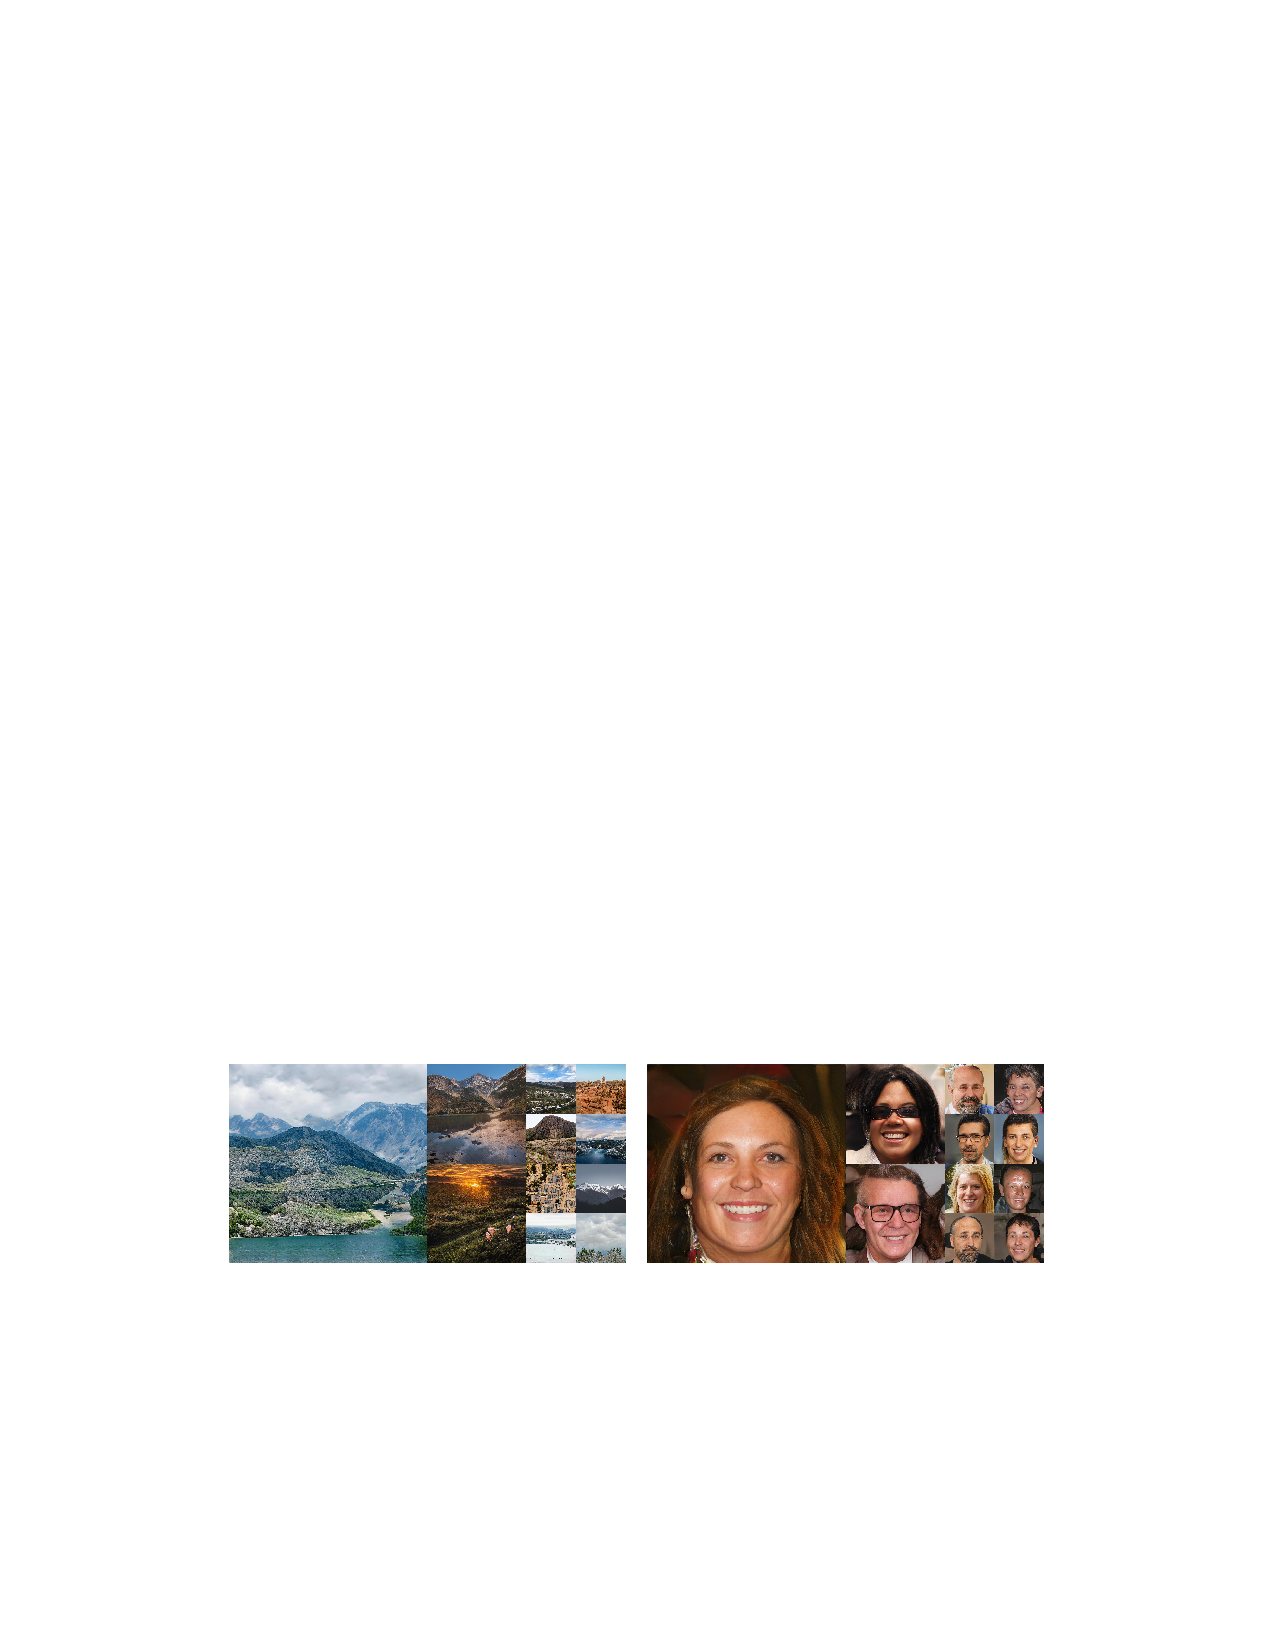
\includegraphics[width=\textwidth]{figures/LWGAN.pdf}
    \caption{轻量级GANs在1024x1024分辨率下的生成效果}
    \label{fig:LWGAN}
\end{figure}

\subsection{损失函数}

我们用$\mathcal{L}_{GAN}(G, D)$表示GANs训练的损失函数。$\mathcal{L}_{GAN}(G, D)$的实现方式涉及到GANs训练的稳定性和生成数据的真实度,因此一直是GANs研究的重点问题。

在原始GANs中,$\mathcal{L}_{GAN}(G, D)$的计算如公式~\ref{eq:js_divergence}所示:

\begin{equation}
    \mathcal{L}_{GAN}(G, D) = E_{x \sim p_{\text {data }}(x)}[\log D(x)]+E_{z \sim p_{z}(z)}[\log (1-D(G(z)))]
    \label{eq:js_divergence}
\end{equation}

该公式本质上是生成数据与真实数据之间的JS散度。公式~\ref{eq:js_divergence}中的目标函数对训练生成器来说存在梯度消失的问题~\cite{review},解决这一问题一般的思路是重新设计目标函数。LSGAN~\cite{lsgan, lsgan2}提出使用最小二乘损失替代JS散度,WGAN~\cite{wgan}提出使用Wasserstein距离度量两个分布间的距离,Hinge损失的基本思想是让正例和负例之间的距离尽量大,最初用于支持向量机(SVM)的优化,后被迁移到GANs的训练~\cite{hinge1,hinge2,hinge3}。

\subsection{生成式对抗网络的训练}

生成器和判别器以一种对抗的方式交替训练,我们以先优化判别器为例,介绍GANs的训练流程。

在每次模型迭代中,我们先以公式~\ref{step_D}优化判别器,注意此时我们固定生成器的权重不变。

\begin{equation}
    \max _{D} V(D, G, R) = \mathcal{L}_{GAN}(G, D)
    \label{step_D}
\end{equation}

然后,我们以公式~\ref{step_G}优化生成器,同样的,此时我们固定判别器的权重不变。

\begin{equation}
    \min _{G} V(D, G, R) = \mathcal{L}_{GAN}(G, D)
    \label{step_G}
\end{equation}

将公式~\ref{step_D}和~\ref{step_G}结合起来,我们就得到了如公式~\ref{overall}所示的GANs总损失。

\begin{equation}
    \min _{G} \max _{D} V(D, G, R) = \mathcal{L}_{GAN}(G, D)
\end{equation}

重复上述步骤,直到生成器生成的图像对人来说足够真实,生成图像的真实度也可以用FID~\cite{fid}等评价指标辅助判断。与其他机器学习模型不同,生成器和判别器的损失并不能直接表明模型的好坏,需要我们通过观察生成图像的质量来判断训练进度。

\subsection{生成图像的评价指标}

我们在这里重点介绍4种生成图像的评价指标,分别是SSIM、FSIM、IS和FID,这些评价指标从不同的角度评估了生成图像的真实性,需要根据具体的任务来选择何时的评价指标。

SSIM(Structural Similarity Index Measure,结构相似性)~\cite{ssim},是一种衡量两张图片结构相似性的指标,最初用于比较无失真图像和压缩后失真影像的相似性,可看作失真影像质量的评价指标,现也用于比较任意两张图像的结构相似性。计算公式如下所示:

\begin{equation}
    \operatorname{SSIM}(x, y)=\frac{\left(2 \mu_{x} \mu_{y}+c_{1}\right)\left(2 \sigma_{x y}+c_{2}\right)}{\left(\mu_{x}^{2}+\mu_{y}^{2}+c_{1}\right)\left(\sigma_{x}^{2}+\sigma_{y}^{2}+c_{2}\right)}
\end{equation}
在这里$x$,$y$表示用于比较的两张图片,$\mu_{x}$是$x$的平均值,$\mu_{y}$为$y$的平均值,$\sigma_{x}^{2}$为的$x$方差,$\sigma_{y}^{2}$为$y$的方差,$\sigma_{x y}$为$x$,$y$的协方差。$c_{1}$与$c_{2}$均为常数,用来维持数值稳定。

FSIM(Feature Similarity Index Measure,特征相似性)~\cite{fsim},概念与SSIM类似,考察两张图像特征的相似性。

IS(Inception Score)~\cite{salimans2016improved}对每张生成图像,使用Inception模型~\cite{inception}计算条件标签分布$p(y|x)$。如果生成图像中包含有意义的物体,那么计算条件标签分布$p(y|x)$的值应该较低。另一方面,我们希望生成图像尽可能多样化,反映在边缘概率$\int p(y \mid x=G(z)) dz$上应该是较大的值。结合上述两点,IS的计算公式为:

\begin{equation}
    IS\left(p(y \mid x), p(y)\right)=\exp \left(E_{x} K L(p(y \mid x) \| p(y))\right)
\end{equation}

更高的IS分数意味着生成器能够生成具有明确语义且多样化的图像。然而,IS分数也有其劣势,如果生成模型陷入模式坍塌,IS分数可能仍然较低。

FID(Fréchet Inception Distance)~\cite{fid}是专为GANs设计的评价指标,计算方式是使用Inception模型的卷积层特征计算函数$\phi$,对真实数据分布$p_{data}$和生成数据分布$p_{g}$建模为高斯随机变量$\phi (p_{data})$和$\phi (p_{g})$,其均值为$\mu_{r}$, $\mu_{g}$,方差为$C_{r}$, $C_{g}$,最后计算:
\begin{equation}
    F I D\left(p_{\text {data }}, p_{g}\right)=\left\|\mu_{r}-\mu_{g}\right\| + tr\left(C_{r}+C_{g}-2\left(C_{r} C_{g}\right)^{1 / 2}\right)
\end{equation}
即可得到FID分数,本质上是这两个高斯分布之间的弗雷歇距离(Fréchet distance)。

\section{生成式对抗网络的应用}

\subsection{图像转换}

图像转换(Image translation)指将输入图像从原风格转换为目标风格(风格转换)或从原图像域转换为目标图像域。 随着深度学习的发展,神经网络风格迁移(neural sytle transfer)~\cite{transfer0,transfer1,transfer2}已经成为风格迁移的主流方法。 风格迁移侧重于不同的艺术风格间的转换,而图像转换~\cite{i2i0,i2i1,i2i2,cyclegan} 解决了更一般的图像域转换问题。

不同的图像转换方法侧重于从不同的角度,解决不同类型的图像转换问题。Pix2Pix~\cite{pix2pix}解决了成对图像(像素对齐的两张图像)的图像转换问题。对于损失函数,Pix2Pix的作者认为可以依靠L1损失约束低频信息,判别器仅用来鉴别高频信息是否真实,作者进一步提出了PatchGAN。 PatchGAN的核心思想是,既然判别器只用于鉴别高频信息,那么就不需要将整张图片输入到判别器中,只在patch(正方形像素块,作者最终采用了70x70的像素块作为patch)的规模上计算高频结构损失。因为不同的patch之间可以认为是相互独立的。PatchGAN对一张图片切割成不同的N x N大小的patch,判别器对每一个patch做真假判别,将一张图片所有patch的结果取平均作为最终的判别器输出。作者认为这会鼓励GANs生成的图像包含清晰的高频细节。

现实世界中更一般的实际上是非成对图像的转换,因为成对图像在大部分真实场景非常难以获取,比如我们要做马和斑马之间的转换,几乎不可能找到像素点对齐的马和斑马的成对图像。
CycleGAN~\cite{cyclegan}提出了循环一致性损失解决了非成对图像的转换问题。与常规的GANs不同,CycleGAN包含两个生成器$G_A$和$G_B$,与两个判别器$D_A$和$D_B$。假设我们有两张分别来自于$A$图像域和$B$图像域的图片$I^A$和$I^B$,非成对图像转换的难点在于,如果我们要将$I^A$转换到$B$域,我们没有$I^A$在$B$域的对应图像,因此无法用类似L1损失的方式约束像素之间的差异。在计算循环一致性损失时,先用$G_A$将$I^A$转换到$B$域,再用$G_B$将上一步的结果转换回$A$域,得到$I^A_{cyc}$,此时就可以计算$I^A$和$I^A_{cyc}$之间的差异,$I^B$和$I^B_{cyc}$的计算类似,如公式~\ref{eq:cyc}所示。

\begin{equation}
    \mathcal{L}_{\mathrm{cyc}}(G, F) =\mathbb{E}_{x \sim p_{\text {data }}(x)}\left[\|F(G(x))-x\|_{1}\right] +\mathbb{E}_{y \sim p_{\text {data }}(y)}\left[\|G(F(y))-y\|_{1}\right]
    \label{eq:cyc}
\end{equation}

无论是Pix2Pix还是CycleGAN,都是解决了两个图像域之间的转换,如果需要多个域之间互相转换,只能训练多个模型,StarGAN~\cite{stargan}通过在输入增加目标域对应的掩码(mask)和类别损失,使用单一模型解决了多个域之间互相转换的问题。

图像转换方法从整体来看,都是输入一张图像,然后转换为另一张图像,与下面要介绍的隐空间编辑方法有很大不同,因此一部分文献~\cite{iclr2021}将图像转换又称为图像空间编辑。目前大多数基于GANs的图像空间编辑方法的问题在于难以同时编辑多个属性,并精确控制生成图像中的属性强度。

\subsection{隐空间编辑}

在GANs发展的早期,Alec Radford等人就在\cite{DCGAN}中发现GANs的隐空间中通常包含有语义意义的向量算法,例如,隐空间中存在能为人脸添加微笑或眼镜的方向。我们称这类通过隐空间向量运算实现图像编辑方法为隐空间编辑方法,区别于上文提到的图像空间编辑方法,后者是对图像直接的转换。

由于隐空间编辑使图像编辑更加简单,因此近些年来这类方法收到越来越多的关注。从隐空间编辑的监督方式来看,隐空间编辑方法分为有监督、无监督、自监督或半监督的方法。

\begin{enumerate}
\item 有监督的隐空间编辑方法采用明确的人工监督来识别隐空间中的可解释方向,如Yujun Shen等人~\cite{interfacegan}使用在CelebA数据集~\cite{celeba}上预训练的二分类器来预测人脸属性。然后使用该分类器为生成的图像及对应的隐变量生成伪标签。基于这些伪标签,可以在隐空间空间中构建分类超平面,该超平面的法线即为相应属性变化的方向。

\item 无监督通过学习一组语义上区别较大的方向~\cite{icml2020} 或基于主成分分析(PCA)的方法~\cite{harkonen2020ganspace}识别潜在的的语义方向。这些方法可能会找到有意义的方向,但其结果是不可预测的,并且需要人工解释,这导致了非监督的隐空间编辑方法难以指定所需的语义方向。

\item 自监督方法~\cite{steer,variation} 通过使用简单的几何变换(例如旋转和缩放)增加数据来搜索可解释的方向,这限制了这些方法搜索复杂属性的能力。
\end{enumerate}

以上方法的本质均是在预训练的GANs的隐空间中搜索语义方向,不可避免地受到预训练GANs的影响,由于GANs在训练时没有受到语义属性的约束,其隐空间必然存在语义耦合现象。这导致现有的隐空间编辑的方法在改变某一属性时,通常会导致其他的属性也发生变化。    

\subsection{多模态图像转换}

在图像处理、计算机视觉和计算机图形学的许多应用中,越来越依赖于多模态医学图像。例如精准医学,脑部核磁共振中存在T1、T1Gd、T2和T2-FLAIR四种模态~\cite{drevelegas2011imaging}。医生希望结合完整的多模态医学图像来做出更精确的诊断,但受限于实际条件限制(例如,受限的医疗条件、扫描时间不足以及成本/支出/资源等限制),实践中可能存在成像系统存在误差,甚至部分模态缺失的现象~\cite{tanenbaum2017synthetic}。这些不可用的图像可能会导致医生决策出现偏差。

Dongwook Lee等人提出的CollaGAN~\cite{collagan}是第一篇将GANs用于多模态图像。与CycleGAN,Pix2Pix等单模态图像转换方法只能输入一种模态的图像不同,CollaGAN针对多模态图像转换提出了多重循环一致损失(Multiple cycle consistency loss),通过一个GANs模型解决了多模态间模态转换的问题。

CollaGAN和使用单个模型在一定程度上解决了多模态图像转换的问题,但没有在训练过程中对模态间的一致性和互补性进行约束。

\section{本章小结}

在本章节我们总结了生成式对抗网络,图片空间编辑、隐空间编辑和多模态图像转换的原理、应用和进展,重点梳理了隐空间编辑和多模态图像现有方法的优势与不足,为后续本文解决方案的提出奠定了基础。
